\begin{figure}
\centering
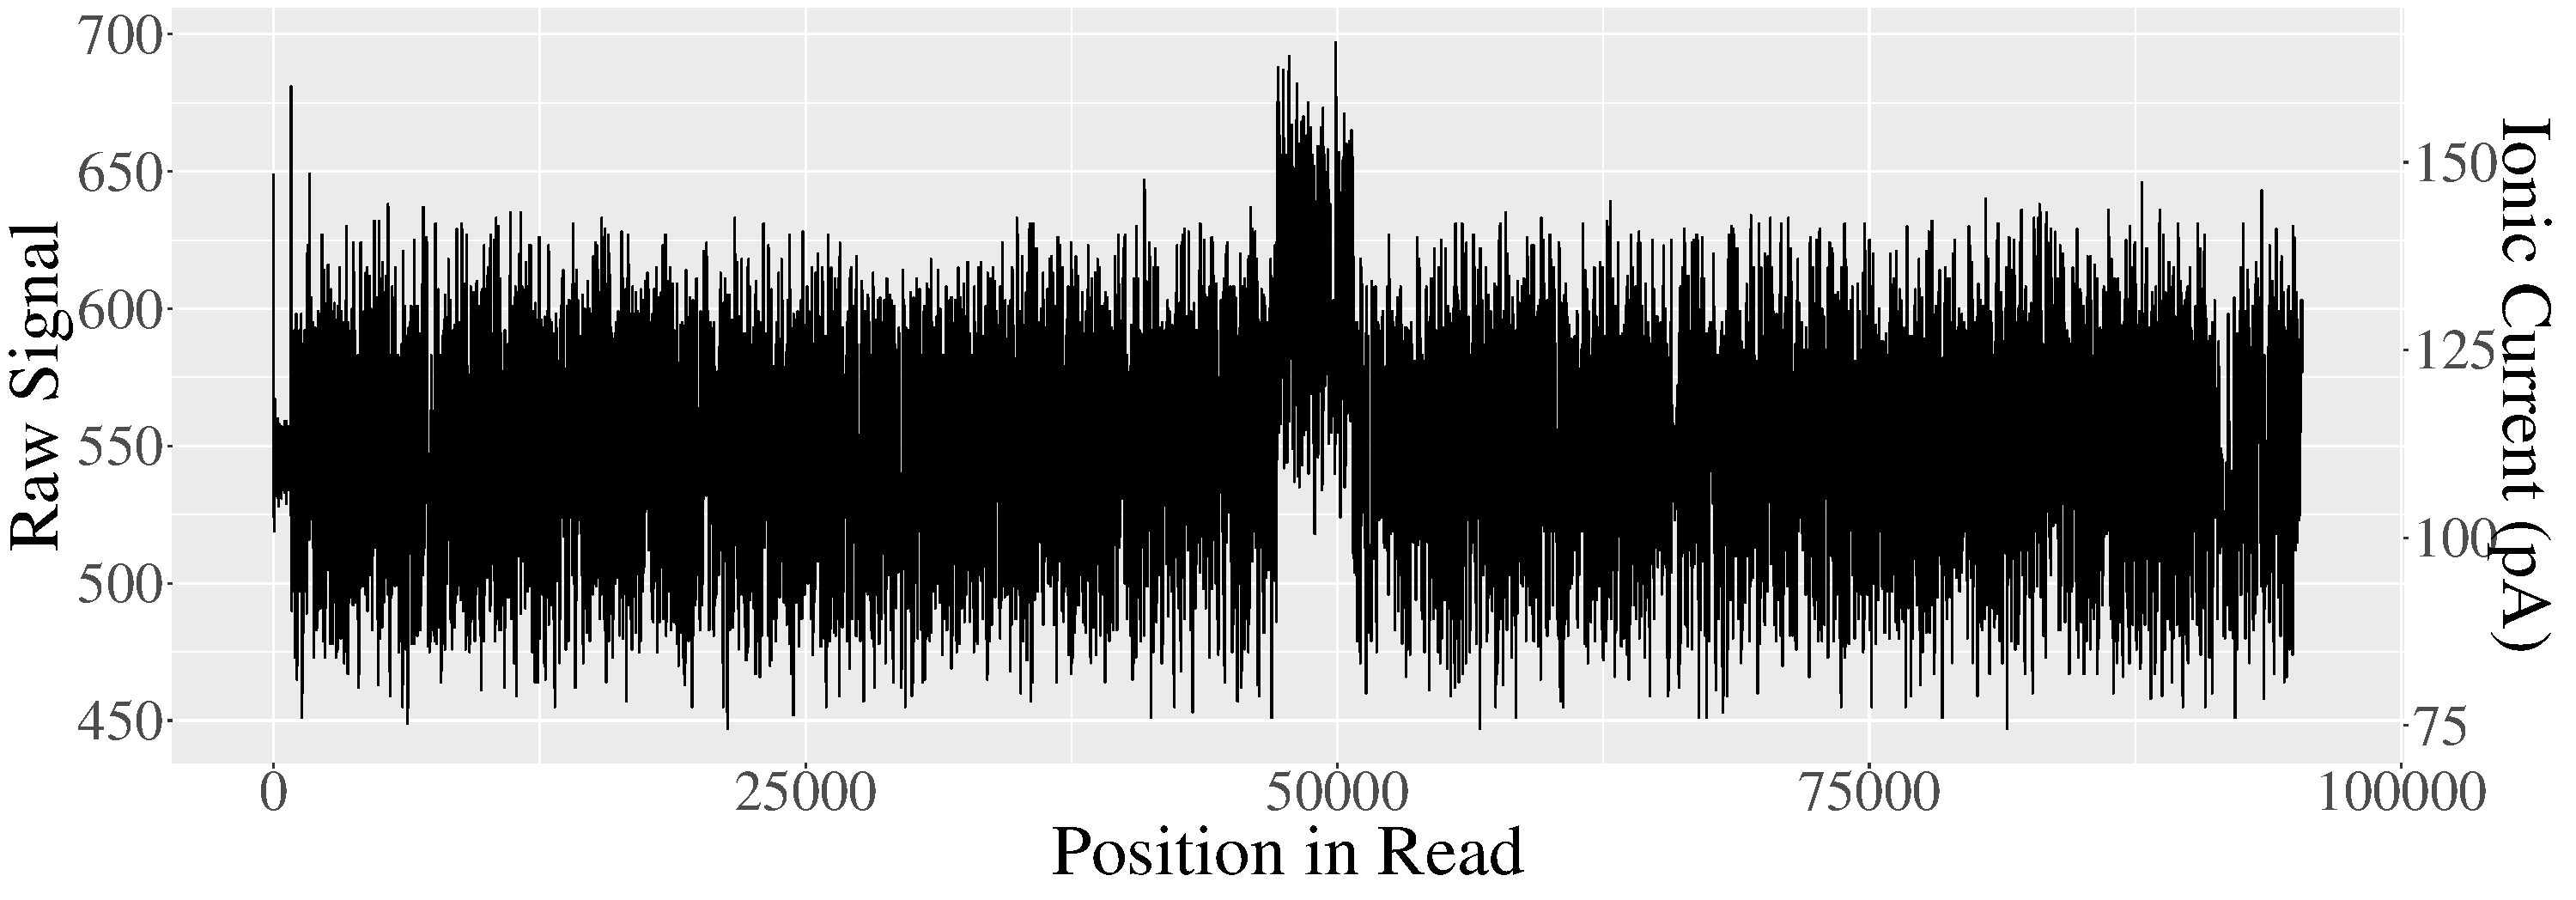
\includegraphics[scale=0.31]{plots/reads.e9f08690-171f-476f-9119-5330d0290126.raw.pa.pdf}
	\caption{\label{fig:read-e9f-pa}The read with ID e9f08690-171f-476f-9119-5330d0290126 from the NA12878 data set plotted against two axes. The primary $y$-axis (left) is the raw signal values and the secondary $y$-axis (right) is the ionic current found using equation \ref{eq:pa}. $535, 531, 529, 519, 535,\dots$ is the sequence starting from position 25000 and $106.73, 105.27, 104.54, 100.88, 106.73,\dots$ is the same sequence after converting to picoamperes (rounded to 2 decimal places).}
\end{figure}
